\documentclass{article}



%========================================
% Packages
%========================================

\usepackage{apacite}
\usepackage{amsmath}            % Formeln
\usepackage{amsfonts}           % Fonts for Formulas
\usepackage{amssymb}
\usepackage[final]{graphicx}
\usepackage{booktabs}
\usepackage{enumerate}
\usepackage{proofing}
\usepackage{txfonts} % for strict implication symbols
\usepackage{multicol}
\usepackage{eurosym}
\usepackage[colorinlistoftodos,color=lightgray,bordercolor=blue,textsize=footnotesize]{todonotes}
\usepackage{tikz}
\usetikzlibrary{backgrounds,fit}
\usepackage{xspace}
\usepackage{subfig}
\usepackage{units}
\usepackage{caption}
\usepackage{tikz}
\usepackage{pgfplots}
\usepackage{wrapfig}
\usepackage{fullpage}
\usepackage{hyperref}
\usepackage{gb4e}


\usepackage{tabularx}
\newcolumntype{R}[1]{>{\raggedleft\arraybackslash}p{#1}}


\pgfdeclarelayer{background}
\pgfdeclarelayer{foreground}
\pgfsetlayers{background,main,foreground}

%========================================
% Color
%========================================
\usepackage{color}
\definecolor{Red}{RGB}{255,0,0}
\definecolor{Blue}{RGB}{0,0,255}
\definecolor{mycol}{RGB}{20,50,200}
\newcommand{\red}[1]{\textcolor{Red}{#1}}
\newcommand{\blue}[1]{\textcolor{Blue}{#1}}
\newcommand{\mygray}[1]{\textcolor{gray}{#1}}
\newcommand{\mycol}[1]{\textcolor{teal}{#1}}

%========================================
% More Layout
%========================================

% Itemize
\renewcommand{\labelitemi}{\large{$\mathbf{\cdot}$}}    % itemize symbols
\renewcommand{\labelitemii}{\large{$\mathbf{\cdot}$}}
\renewcommand{\labelitemiii}{\large{$\mathbf{\cdot}$}}
\renewcommand{\labelitemiv}{\large{$\mathbf{\cdot}$}}

% Description
\renewcommand{\descriptionlabel}[1]{\hspace\labelsep\textsc{#1}}

\title{Notes on sinking marbles}

\author{Judith Degen}

%========================================
% Document
%========================================


%\renewcommand{\familydefault}{\sfdefault}
\begin{document}

\maketitle

\tableofcontents

\section{Motivation}

From Bart Geurts's book ``Quantity Implicatures'':
\blue{``The cancellation argument presupposes that preferred scalar inferences will quietly withdraw whenever they happen to be implausible, and this pre- supposition is doubtful, as it is contradicted by the behaviour of bona fide scalar inferences. Let me give a couple of examples to establish this point.}

\begin{exe}
	\ex \blue{Some of the liberal parliamentarians voted against the bill.}
\end{exe}

\blue{In some democracies, parliamentary fractions tend to vote en bloc. In the Netherlands, for instance, it would be quite unlikely that some but not all liberal parliamentarians voted against a bill. Nevertheless, as far as I can tell, this wouldn�t diminish the likelihood that (58) is interpreted as implying that the liberal fraction was divided.}

\begin{exe}
	\ex \blue{In order to prevent the rinderpest from spreading through the herd, some of the cows were vaccinated.}
\end{exe}

\blue{Since rinderpest is a highly contagious disease, it would be decidedly odd if only some of the cows were vaccinated, yet that is how we would understand (59).}

\begin{exe}
	 \ex \blue{Cleo threw all her marbles in the swimming pool. Some of them sank to the bottom.}
\end{exe}

 \blue{No doubt, it would be very odd if some of Cleo�s marbles failed to sink, yet according to my intuitions that is precisely what (60) conveys.}

 \blue{What these examples show is that genuine scalar inferences are not so easy to cancel, at all (cf. Geurts 1999a). From a Gricean perspective, this is to be expected: scalar implicatures arise because the speaker goes out of his way to make a statement that is weaker than what he could have said with equal effort, so it stands to reason that it should require special circumstances to suppress a scalar implicature. But in particular, lack of plausibility will generally be insufficient for doing so."}

\bigskip

Our questions are: do Bart's intuitions pan out empirically? And if so, how can we model this effect? 

General modeling idea: if the prior probability of the $\forall$ state is high enough and there's a cheap enough alternative utterance --say, silence, or in order to refer to it: \emph{null}-- to \emph{some} (crucially, cheaper than \emph{some}) that signifies something like ``everything is as usual'', then the fact that the speaker went to the (extra) effort of saying \emph{some} instead of \emph{null} means things must really be different than the normal case. But if the normal case is $\forall$, then by saying \emph{some} the speaker must really mean $\exists \wedge \neg \forall$. That is, there are two counter-acting forces: a) higher prior probability of $\forall$ state \emph{increases} the posterior probability of $\forall$ state after observing \emph{some}; b) presence of \emph{null} alternative \emph{decreases} posterior probability of $\forall$ state after observing \emph{some} (if prior probability of $\forall$ is very high (\red{how high is an empirical question})).

A preliminary version of the model is here: \url{http://forestdb.org/models/SFVSome.html} It's got some unnecessary bits leftover from when the model was intended to capture QUD effects. The general shape of the posterior curve for $\forall$ that it predicts is shown in Figure \ref{fig:model-predictedshape}.


\begin{figure}
	\begin{center}
	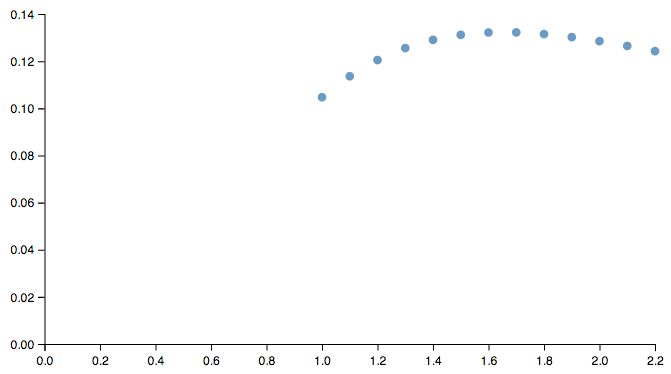
\includegraphics[width=.8\textwidth]{pics/model-predictedshape.png}
	\end{center}
	\caption{Model predictions for $\forall$ state after observing \emph{Some of the X sank} with different prior probabilities of $\forall$ state (i.e.~different X types) on the x-axis. Plot generated in play-space with alternative weights for \emph{null; none; some; all} $=$ 20; 1; 1; 1.}
	\label{fig:model-predictedshape}
\end{figure}

\section{Experiment 1 - preliminary pilot}

The experiment can be found here: \url{http://stanford.edu/~jdegen/57_sinkingmarbles/alternatives.html}

\subsection{Method}

\subsubsection{Participants}
30 participants were recruited over Amazon's Mechanical Turk. 

\subsubsection{Procedure and materials}

The experiment consisted of two phases: prior and posterior elicitation. The prior phase was intended to assess participants' prior beliefs about how likely different types of objects are to either \emph{break/sink} prior to observing any additional information. Object types were marbles, feathers, balloons, books, wine glasses, iPhones. See Figure \ref{fig:priortrial} for an example of a prior trial (including slider dependent measure).

\begin{figure}
	\begin{center}
	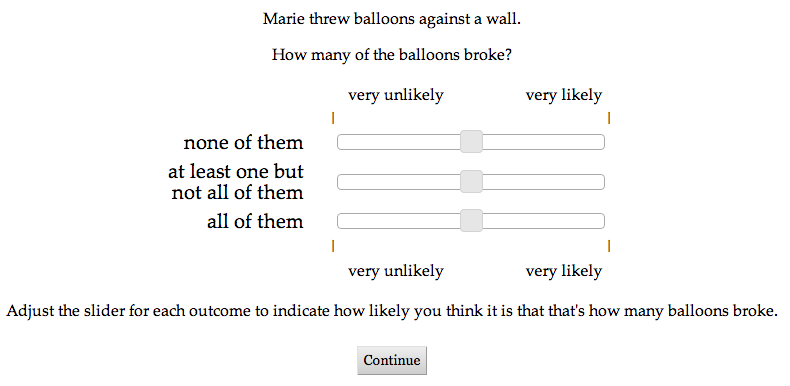
\includegraphics[width=\textwidth]{pics/priortrial.png}
	\end{center}
	\caption{Example of a display in the prior elicitation phase.}
	\label{fig:priortrial}
\end{figure}

\begin{figure}
	\begin{center}
	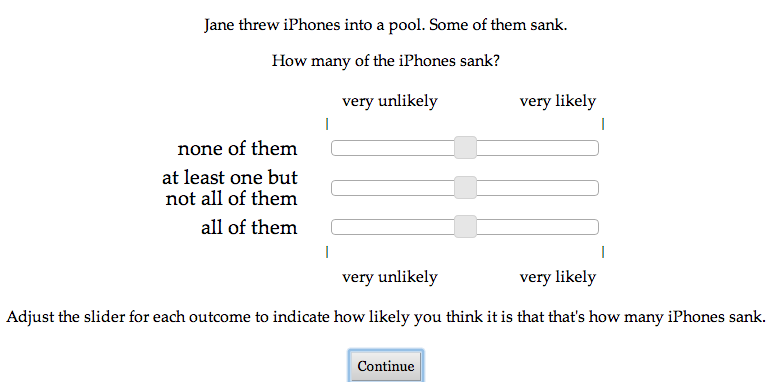
\includegraphics[width=\textwidth]{pics/posteriortrial.png}
	\end{center}
	\caption{Example of a display in the posterior elicitation phase.}
	\label{fig:posteriortrial}
\end{figure}

In the posterior elicitation phase, additional information about how many of the objects sank/broke was given by adding an additional sentence: either \emph{All} or \emph{Some of the X broke/sank}. See Figure \ref{fig:posteriortrial} for an example of a posterior trial.

Each phase of the experiment consisted of 12 trials: each of the six object types occurred with each verb (break/sink) in each phase. In the posterior phase, an object occurred once with \emph{all} and once with \emph{some}, but \emph{all/some} were randomly paired with \emph{break/sink}. That is, for each combination of verb/object we obtained 30 prior probabilities and for each verb/object/quantifier combination we obtained 15 posterior probabilities.

\subsection{Results}

Slider values were normalized for each trial to yield a probability distribution over states $\neg \exists$, $\exists \wedge \neg \forall$, and $\forall$ for each verb/object combination in the prior phase and each verb/object/quantifier combination in the posterior phase. Figure \ref{fig:all-prior} shows the mean prior probabilities of the $\forall$ state for each object/verb combination.

\begin{figure}
	\begin{center}
	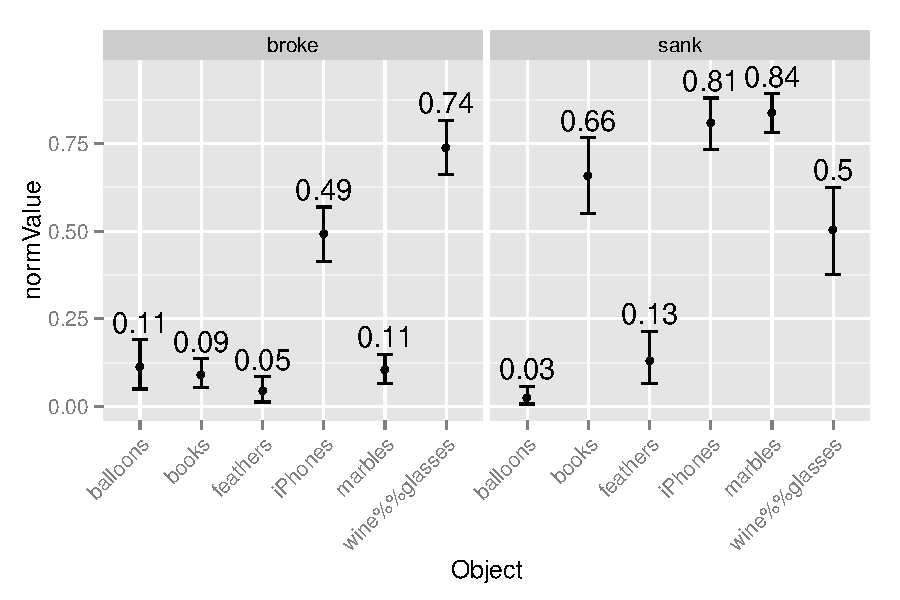
\includegraphics[width=.8\textwidth]{pics/all-prior}
	\end{center}
	\caption{Mean prior probability of all objects breaking (left) or sinking (right) by object type.}
	\label{fig:all-prior}
\end{figure}



The interesting question was whether we would see something like the shape in Figure \ref{fig:model-predictedshape}. The empirical results are shown in Figure \ref{fig:empirical-results} (unaggregated) and Figure \ref{fig:posterior-aggr}.

\begin{figure}
	\begin{center}
	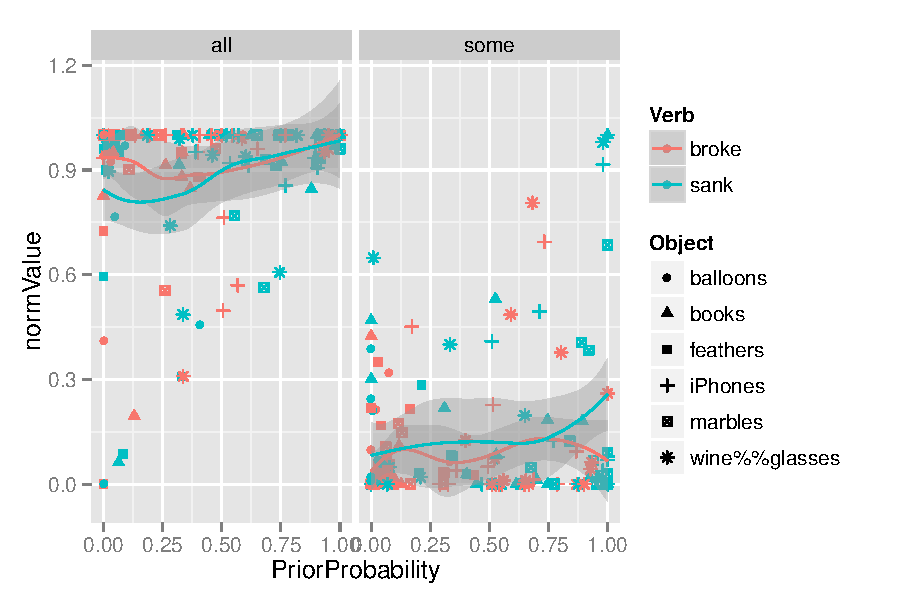
\includegraphics[width=.9\textwidth]{pics/empirical-results}
	\end{center}
	\caption{Posterior probability of each object breaking/sinking after being informed that \emph{all} (left) or \emph{some} (right) of them broke, by unaggregated (by-subject) prior probability of all of them breaking/sinking.}
	\label{fig:empirical-results}
\end{figure}

\begin{figure}
	\begin{center}
	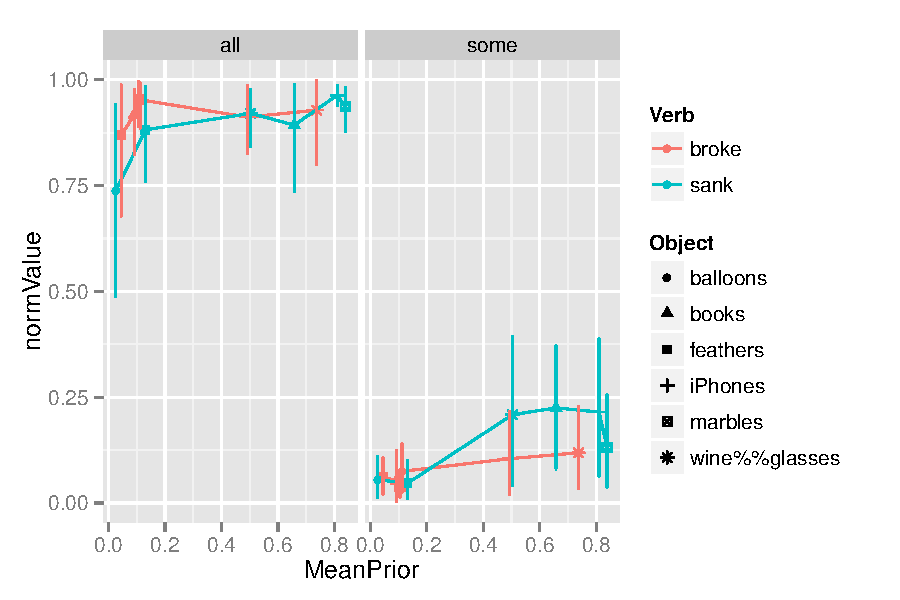
\includegraphics[width=.9\textwidth]{pics/posterior-aggr}
	\end{center}
	\caption{Posterior probability of each object breaking/sinking after being informed that \emph{all} (left) or \emph{some} (right) of them broke, by aggregated prior probability of all of them breaking/sinking. Error bars indicate bootstrapped 95\% confidence intervals.}
	\label{fig:posterior-aggr}
\end{figure}

\subsection{Discussion}

The unaggregated data look super noisy, the aggregated ones seem to at least sort of show the right shape in the \emph{sink} but not the \emph{break} condition, but the error bars are huge. That it doesn't show up even a little bit in the \emph{break} condition might be because none of the object types has a prior probability of breaking that's high enough (the highest we got was .74 for wine glasses). 

Generally we have the problem so far that we're over-sampling the low- and under-sampling the high-prior-probability space. That is, we need more object types with a better spread, and preferably clustered around the higher range.

Another thing: one of the reasons the results might be so noisy is that the \emph{all/some} information is not presented as part of a speaker's utterance, but as part of the instructions on each trial.

So\dots

\section{Experiment 2 - prior elicitation}

The goal of this experiment was to pilot a series of items and make sure there was a large range of prior probabilities for different events and especially, that we got many samples from the highest region, i.e.~probability$>$.8. The experiment can be found here: \url{https://web.stanford.edu/~erindb/sinking-marbles/experiments/sinking-marbles-prior/sinking-marbles-prior.html}

\subsection{Method}

\subsubsection{Participants}
60 participants were recruited over Amazon's Mechanical Turk and paid \$0.50 each. 

\subsubsection{Procedure and materials}

On each trial, participants saw a display as in Figure \ref{fig:priorpilot}, which consisted of a sentence frame ``SPEAKER VERB-ed 100 OBJECTs EXTRA'', e.g.~\emph{Mary threw 100 cakes against a wall}. They were then asked to provide an estimate for how many OBJECTs displayed a certain EFFECT, e.g.~sticking to the wall, by adjusting a slider.

\begin{figure}
	\begin{center}
	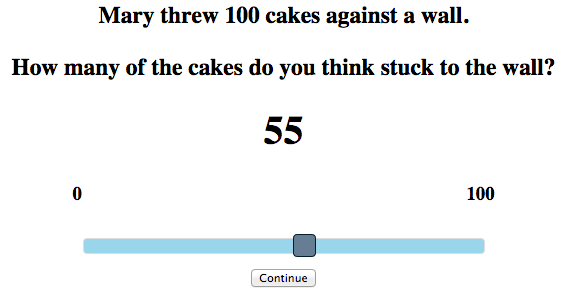
\includegraphics[width=.8\textwidth]{pics/priorpilot}
	\end{center}
	\caption{Display in prior elicitation experiment 2.}
	\label{fig:priorpilot}
\end{figure}

Three items were created for each VERB-EXTRA combination, corresponding to three different OBJECT types. OBJECT types were chosen in such a way as to result in low, medium, and high prior probabilities of displaying the EFFECT. Each participant saw each VERB-EXTRA combination with only one OBJECT type. Each participant saw a total of 30 trials.

\subsection{Results}

See Figures \ref{fig:exp2-histogram} and \ref{fig:exp2-distribution}.

\begin{figure}
	\begin{center}
	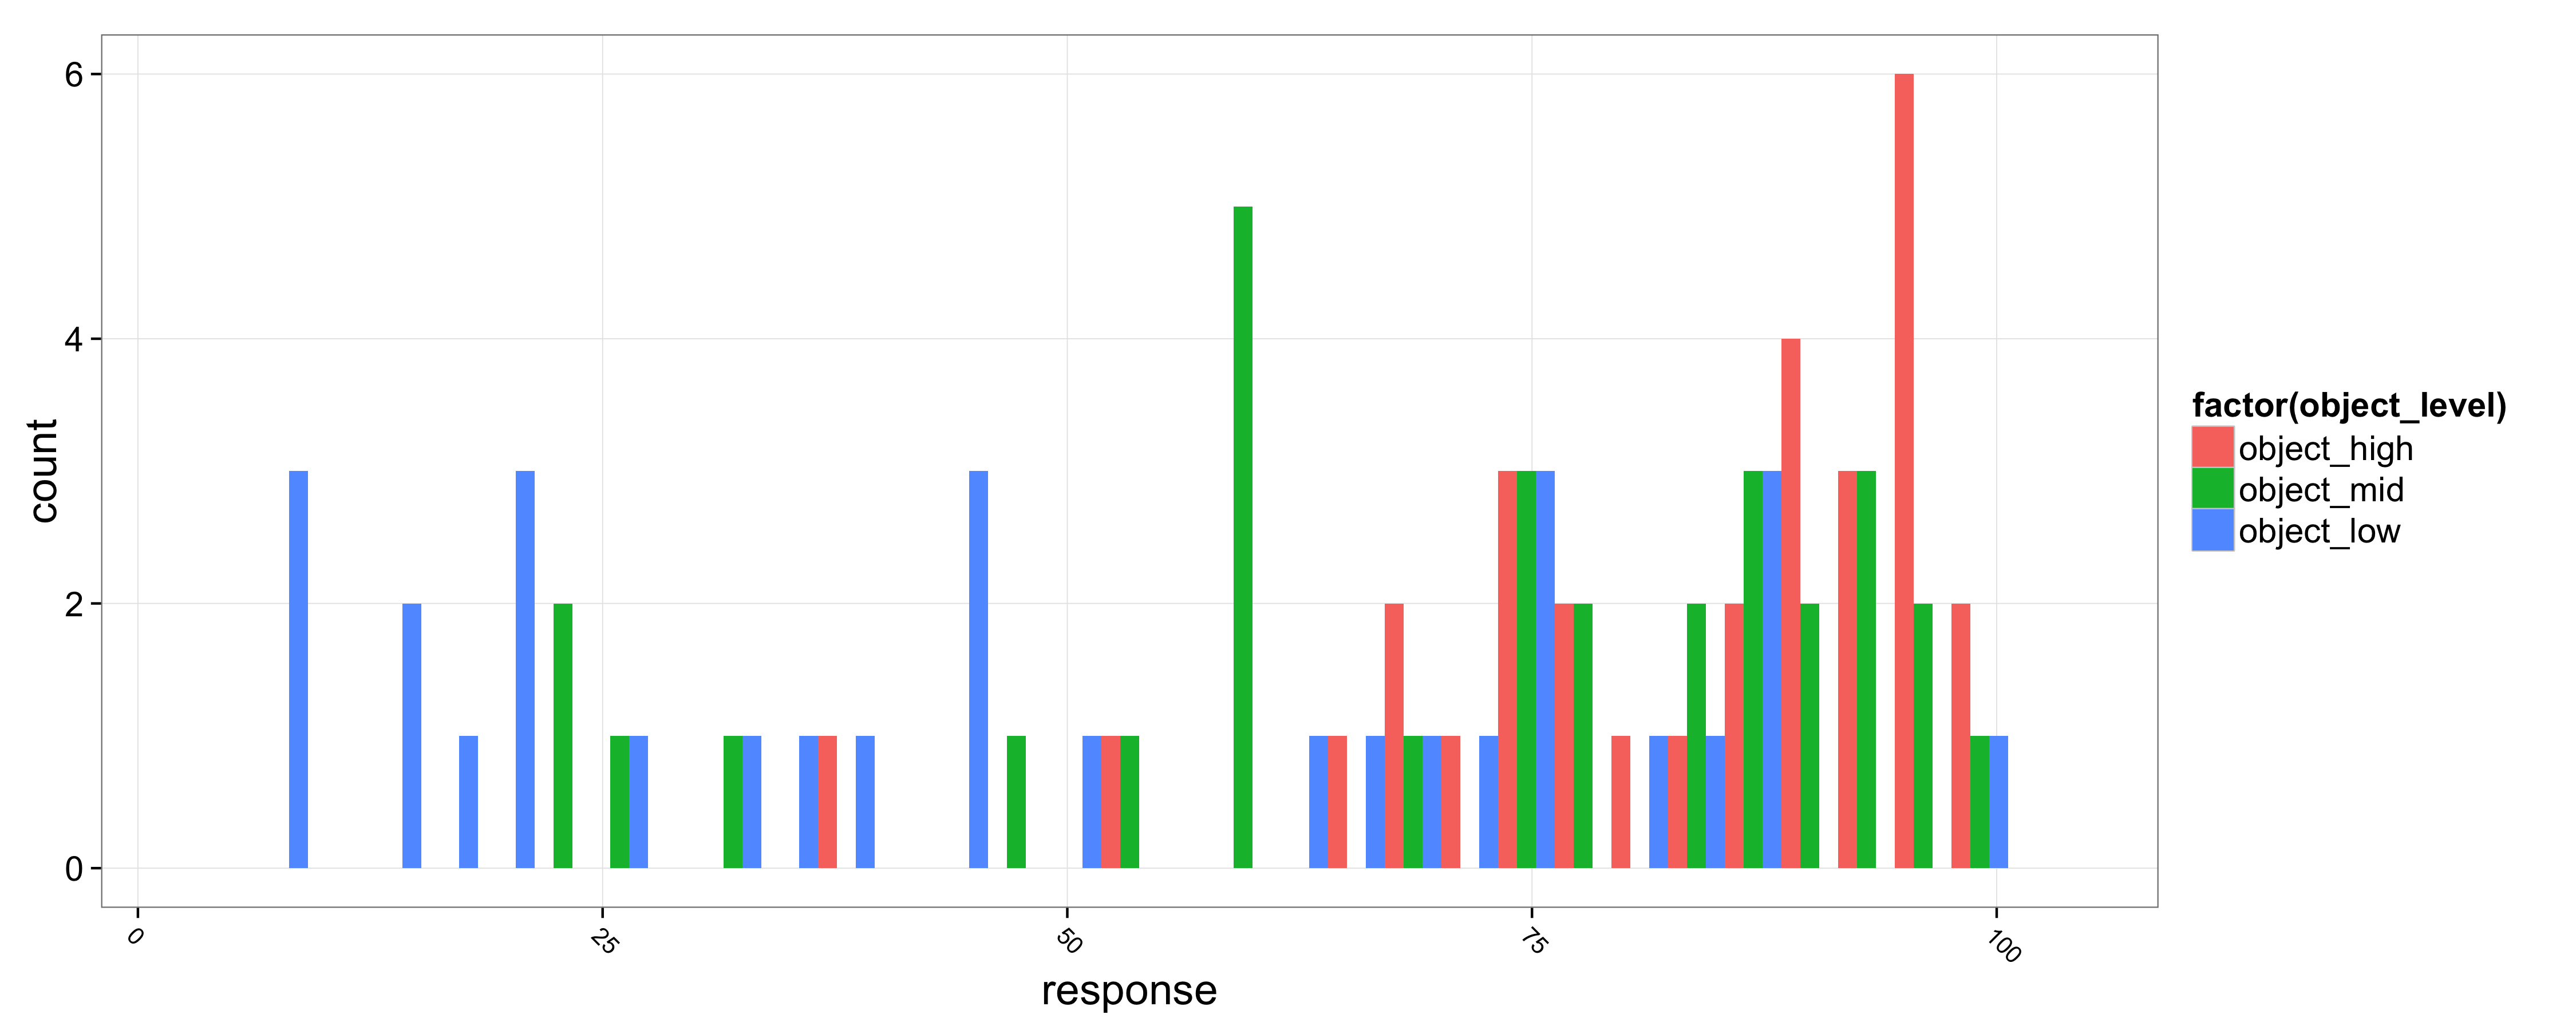
\includegraphics[width=\textwidth]{pics/exp2-histogram}
	\end{center}
	\caption{Histogram of elicited mean priors.}
	\label{fig:exp2-histogram}
\end{figure}

\begin{figure}
	\begin{center}
	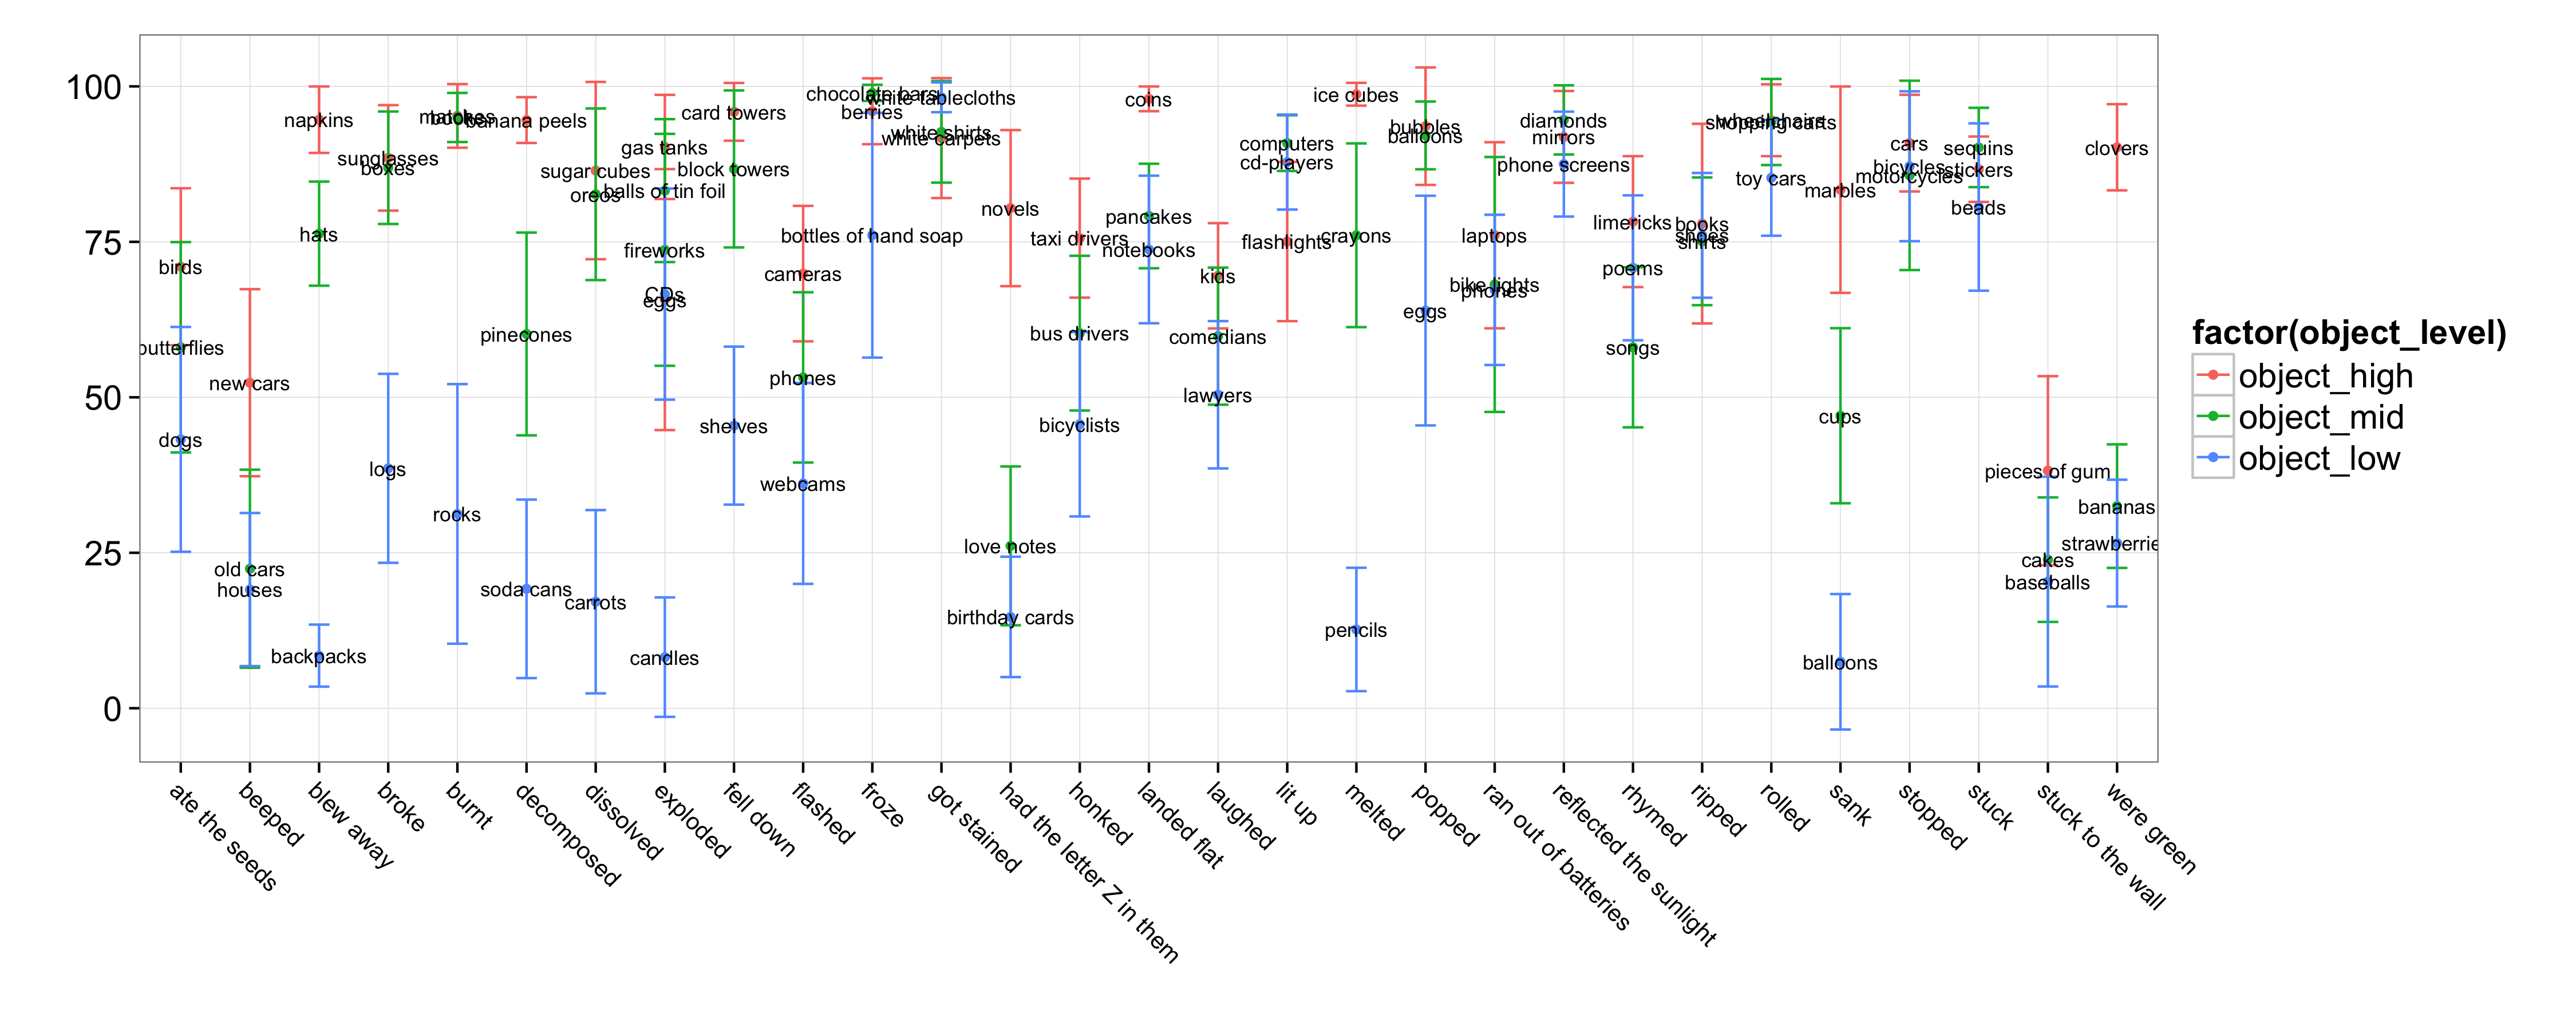
\includegraphics[width=\textwidth]{pics/exp2-distribution}
	\end{center}
	\caption{Elicited mean priors by object type.}
	\label{fig:exp2-distribution}
\end{figure}


\subsection{Discussion}

This is a nice range and especially covers the highest end of the spectrum. Some of the items displayed some idiosyncrasies -- issues of EFFECT being a state/inherent property rather than a point outcome (accomplishment or whatever the linguists call it). And differences in how long the agent needs to be present to observe the EFFECT. Does it matter? Let's assume for the time being it doesn't. 


\section{Experiment 3 - sinking marbles, version 1}

The goal of this experiment was to test for the predicted `sinking marbles' effect. The experiment can be found here: \url{https://web.stanford.edu/~erindb/sinking-marbles/experiments/sinking-marbles/sinking-marbles-prior.html}

\subsection{Method}

\subsubsection{Participants}
120 participants were recruited over Amazon's Mechanical Turk and paid \$??? each. 

\subsubsection{Procedure and materials}

On each trial, participants saw a display as in Figure \ref{fig:sinkingmarbles-display}, which consisted of a sentence frame ``PERSON VERB-ed N OBJECTs EXTRA'', e.g.~\emph{Mary threw 12 cakes against a wall}. They were also told that a SPEAKER, who observed what happened, produced an utterance. The utterance was always of the form ``QUANTIFIER of the OBJECTs EFFECT.'', e.g.~\emph{All of the cakes stuck to the wall}. They were then asked to provide an estimate for how many OBJECTs displayed the EFFECT, e.g.~sticking to the wall, by adjusting a slider for each of 4 options: 0\%, 1-50\%, 51-99\%, or 100\%.

\begin{figure}
	\begin{center}
	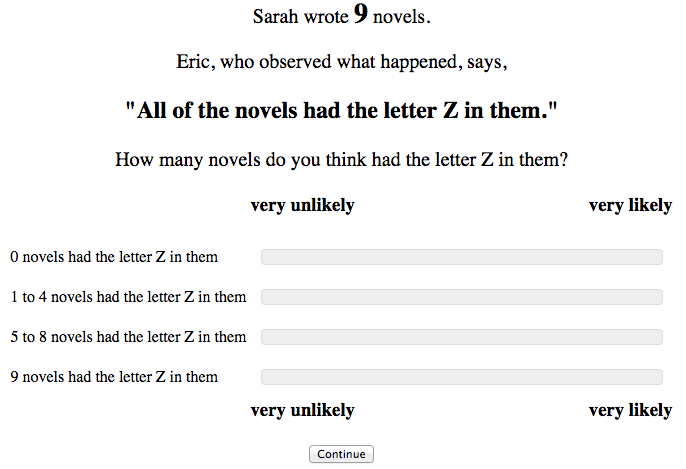
\includegraphics[width=.8\textwidth]{pics/sinkingmarbles-display}
	\end{center}
	\caption{Display in sinking marbles experiment 3.}
	\label{fig:sinkingmarbles-display}
\end{figure}

The same items were used as in Exp.~2. Each participant saw each VERB-EXTRA combination with only one OBJECT type and one QUANTIFIER. QUANTIFIER could be one of \emph{all, most, some} or \emph{none}, and was randomized. N varied randomly from 4 to 15. PERSON and SPEAKER also varied randomly. Each participant saw a total of 30 trials.

\subsection{Results}

We were interested in testing the model prediction that when observing an utterance with \emph{some} a) the probability of the all-state obtaining should increase with increasing  prior probability, and b) the probability of the all-state obtaining should flatten out/decrease again for the highest-prior events because of the availability of saying something cheap or nothing that signals ``everything is as usual''. 

First, sliders were normalized to give a proper probability distribution over proportions (0, .01-.5, .51-.99, 1) on every trial. Figure \ref{fig:exp3-normalized} shows the smoothed mean posterior probabilities as a function of prior probability, separately for each quantifier and proportion. 

\begin{figure}
	\begin{center}
	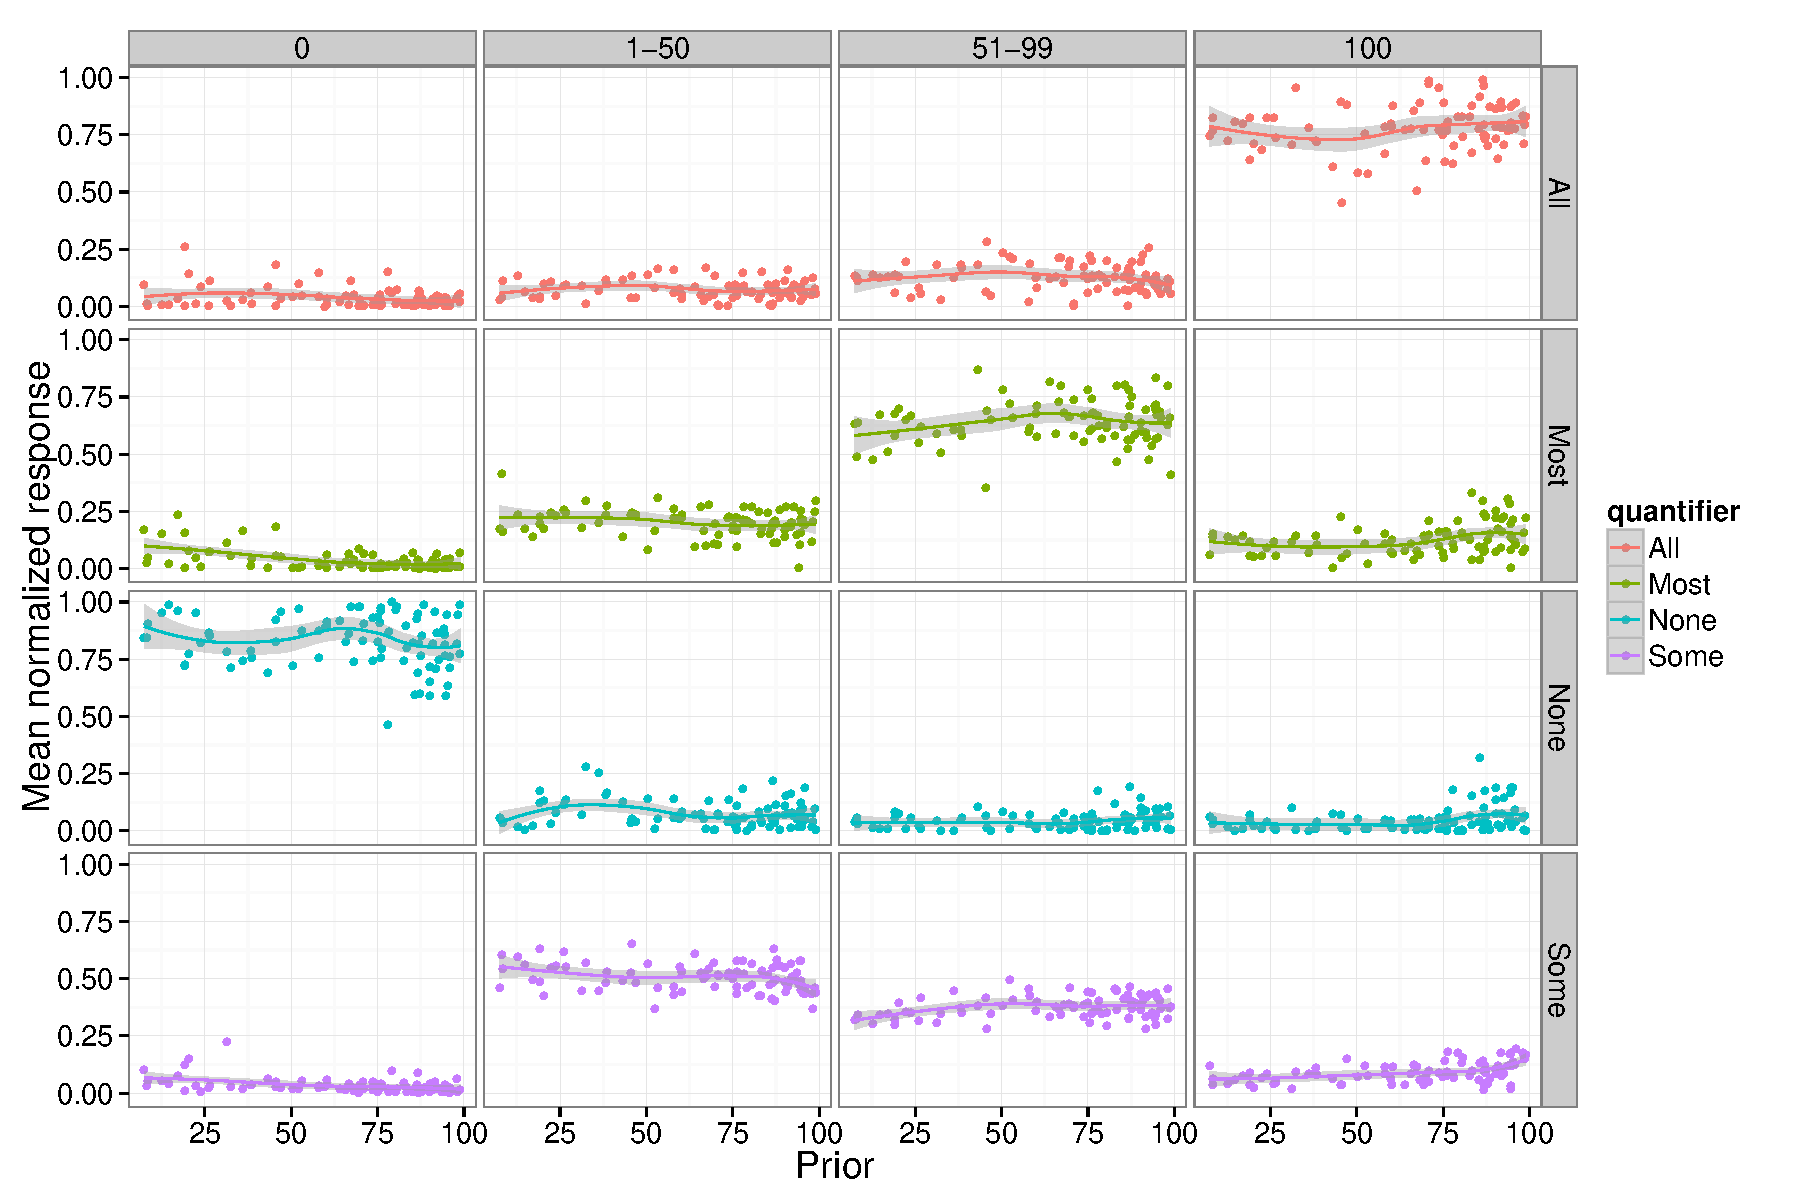
\includegraphics[width=\textwidth]{pics/exp3-normalized}
	\end{center}
	\caption{Smoothed mean posterior probabilities as a function of prior probability, separately for each quantifier and proportion.}
	\label{fig:exp3-normalized}
\end{figure}



\subsection{Discussion}

The interesting column is the last one (100\%), which shows the mean by-item probability of the all-state obtaining. First thing to notice: effect of prior is super small. There's definitely a positive slope for both \emph{some} and \emph{most}, but it's a tiny effect. As for the flattening out effect - it seems to be there for \emph{most}, but not for \emph{some}. Splitting results up by quarter (which really shouldn't be done because there's not enough data...) indicates that whatever effect there is, it's stronger in the first quarter than in the others, where things are just flat. 

So...


\section{To do}

run a version with the following features:
\begin{itemize}
	\item no \emph{most} (because that might be eating up some of the dynamic range we'd otherwise get for \emph{some})
	\item two types of fillers to mimic a null alternative (because people may be restricting the set of alternatives to just sentences of the form ``Q of the O VERB-ed'', but that defeats the purpose of assuming they're entertaining a null alternative): short fillers of the sort ``Typical/normal/nothing out of the ordinary'' and other generic things that signal that \emph{everything is as usual/expected}. And long fillers that basically shift the QUD away from ``How many OBJECTs VERBed?'', thus signaling that it's not the quantity of the OBJECTs that VERBed that's interesting --that's as usual-- but rather something else.

\end{itemize}

\end{document}